\documentclass[../../main.tex]{subfiles}

\begin{document}
\problem{34}
\begin{wts}
What is the IP address of your computer?
\end{wts}
\begin{proof}
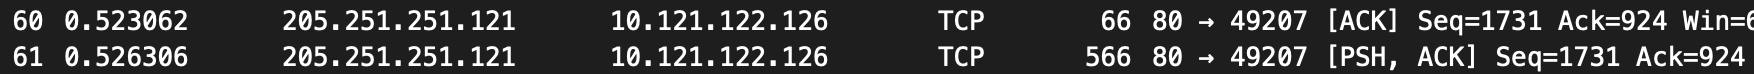
\includegraphics{subfiles/images/ECSE_308_Lab_5_1_SUPA_PAGE4_15_Image48.png}
\subfile{./assorted/Theorem2_14.tex}
\subfile{./assorted/Theorem2_1.tex}
\end{proof}
\begin{wts}
    Show that the set of subsequential limits, denoted by $\szz$ is closed.
\end{wts}
\begin{proof}
    We will prove this by showing that the complement of $\szz$ is open. Indeed, suppose by contradiction that $\szz^c$ is not open. There exists $a\in\szz^c$ such that for every $h^{-1}>0$, (where $h$ ranges through the counting numbers), $V_{h^{-1}}(a)$ is not a subset of $\szz^c$. So there exists a $L_h\in\szz\cap V_{h^{-1}}(a)$, where $L_h$ is a subsequential limit of $x_n$.\\
    
    It is clear that $x_n\in V_{h^{-1}}(L_h)$ for some $L_h\in V_{h^{-1}}(a)$ frequently. To construct a subsequence of $x_n$ that converges to $a$, choose $x_{n_1}$ arbitrarily. It is obvious that for every $h\geq2$, the following set is non-empty,
    \[\mathcal{N}(h)=\biggl\{n\in\nat^+,\,x_n\in V_{h^{-1}}(L_h)\biggr\}\setminus[1,n_{h-1}]\]
    Choose $n_h=\least\mathcal{N}(h)$ inductively, and $x_{n_h}\to a$. Fix any $\varepsilon>0$, and $d(x_{n_h},a)\leq d(x_{n_h},L_h) + d(a, L_h)<2h^{-1}<\varepsilon$
    eventually.
\end{proof}

\end{document}